%%%%%%%%%%%%%%%%%%%%%%%%%%%%%%%%%%%%%%%%%%%%%%%%%%%%%%%%%%%%%%%
% IMPORTANTE: compilar con XeLaTeX (fontspec lo requiere).      %
% Presentación en Beamer (16:9) sobre el informe:               %
% "Predicción de la demanda eléctrica horaria a 24 horas:       %
%  Alemania, España y Francia (2015-2019)".                     %
%                                                                %
% Reutiliza únicamente las figuras y tablas ya preparadas en    %
% reports/presentacion/img/ y reports/presentacion/generated/   %
% (ver reports/presentacion/README.md para el inventario). No   %
% se regenera ningún recurso ni se vuelve a entrenar nada aquí. %
%%%%%%%%%%%%%%%%%%%%%%%%%%%%%%%%%%%%%%%%%%%%%%%%%%%%%%%%%%%%%%%
\documentclass[11pt,aspectratio=169]{beamer}
%%%%%%%%%%%%%%%%%%%%%%%%%%%%%%%%%%%%%%%%%%%%%%%%%%%%%%%%%%%%%%%
% IMPORTANTE: compilar con XeLaTeX (fontspec lo requiere).      %
% Preámbulo de estilo para la presentación en Beamer (16:9),    %
% diseño académico sobrio para proyección en una sala mediana.  %
% Se importa desde main.tex con %%%%%%%%%%%%%%%%%%%%%%%%%%%%%%%%%%%%%%%%%%%%%%%%%%%%%%%%%%%%%%%
% IMPORTANTE: compilar con XeLaTeX (fontspec lo requiere).      %
% Preámbulo de estilo para la presentación en Beamer (16:9),    %
% diseño académico sobrio para proyección en una sala mediana.  %
% Se importa desde main.tex con %%%%%%%%%%%%%%%%%%%%%%%%%%%%%%%%%%%%%%%%%%%%%%%%%%%%%%%%%%%%%%%
% IMPORTANTE: compilar con XeLaTeX (fontspec lo requiere).      %
% Preámbulo de estilo para la presentación en Beamer (16:9),    %
% diseño académico sobrio para proyección en una sala mediana.  %
% Se importa desde main.tex con \input{style}.                  %
%%%%%%%%%%%%%%%%%%%%%%%%%%%%%%%%%%%%%%%%%%%%%%%%%%%%%%%%%%%%%%%

%----------------------------- IDIOMA Y FUENTES ---------------------------
\usepackage[spanish,provide=*,es-noshorthands]{babel}
\selectlanguage{spanish}

\usepackage{fontspec}
% Fuente profesional opcional (requiere tenerla instalada). Por defecto se
% usa la fuente sans-serif estándar de XeLaTeX (Latin Modern Sans), que no
% requiere instalación adicional. Para activar otra, descomentar:
% \setsansfont{Lato}
% \setmainfont{Lato}

%----------------------------- PAQUETES BASE ---------------------------
\usepackage{graphicx}
\usepackage{booktabs}
\usepackage{tabularx}
\usepackage{array}
\usepackage{xcolor}
\usepackage{amsmath,amssymb}
\usepackage{siunitx}
\usepackage{tikz}
\usetikzlibrary{arrows.meta,positioning}
\usepackage{enumitem}

%----------------------------- PALETA (Okabe-Ito, igual que las figuras) ---
\definecolor{navy}{HTML}{1B2A4A}           % títulos
\definecolor{grafito}{HTML}{3C3C3C}        % texto
\definecolor{azulacento}{HTML}{0072B2}     % DE / Ridge / entrenamiento
\definecolor{naranjaacento}{HTML}{E69F00}  % M2 / validación
\definecolor{verdeacento}{HTML}{009E73}    % M3
\definecolor{grisreferencia}{HTML}{999999} % referencias
\definecolor{naranjaoscuro}{HTML}{D55E00}  % M3* cíclico / FR

%----------------------------- TEMA BASE (sin decoraciones) ---------------
\usetheme{default}
\usecolortheme{default}
\setbeamertemplate{navigation symbols}{}
\setbeamertemplate{blocks}[rounded][shadow=false]
\setbeamertemplate{itemize items}[circle]
\setbeamertemplate{enumerate items}[default]
\setbeamertemplate{headline}{} % sin barra superior

\setbeamercolor{background canvas}{bg=white}
\setbeamercolor{normal text}{fg=grafito,bg=white}
\setbeamercolor{structure}{fg=azulacento}
\setbeamercolor{title}{fg=navy}
\setbeamercolor{subtitle}{fg=grafito}
\setbeamercolor{frametitle}{fg=navy,bg=white}
\setbeamercolor{section in head/foot}{fg=grisreferencia,bg=white}
\setbeamercolor{page number in head/foot}{fg=grisreferencia,bg=white}
\setbeamercolor{itemize item}{fg=azulacento}
\setbeamercolor{itemize subitem}{fg=verdeacento}
\setbeamercolor{enumerate item}{fg=azulacento}
\setbeamercolor{alerted text}{fg=naranjaoscuro}
\setbeamercolor{block title}{fg=navy,bg=white}
\setbeamercolor{block body}{fg=grafito,bg=white}
\setbeamercolor{caption name}{fg=grisreferencia}

%----------------------------- TIPOGRAFÍA -----------------------------
% Tamaños relativos de Beamer (no \fontsize absolutos): la página de Beamer
% en aspectratio=169 es un lienzo pequeño (160mm x 90mm) que se amplifica al
% proyectarse, por lo que \fontsize{30}{36}pt literales (pensados para una
% hoja impresa normal) desbordan el frame. Se usan los comandos relativos
% estándar de LaTeX/Beamer, escalados desde el \\documentclass[11pt]{beamer}.
\setbeamerfont{title}{size=\Huge,series=\bfseries}
\setbeamerfont{subtitle}{size=\large}
\setbeamerfont{frametitle}{size=\LARGE,series=\bfseries}
\setbeamerfont{normal text}{size=\normalsize}
\setbeamerfont{itemize/enumerate body}{size=\normalsize}
\setbeamerfont{itemize/enumerate subbody}{size=\small}
\setbeamerfont{block title}{size=\small,series=\bfseries}
\setbeamerfont{block body}{size=\footnotesize}
\setbeamerfont{caption}{size=\footnotesize}
\setbeamerfont{footline}{size=\tiny}
\renewcommand{\arraystretch}{1.25}
% Listas compactas: el espaciado por defecto de itemize/enumerate en Beamer
% es generoso y, acumulado en varios ítems, desborda el cuerpo del frame.
\setlist[itemize]{itemsep=2pt,topsep=2pt,parsep=0pt}
\setlist[enumerate]{itemsep=2pt,topsep=2pt,parsep=0pt}

%----------------------------- MÁRGENES Y PIE DE PÁGINA -----------------
\setbeamersize{text margin left=1.1cm,text margin right=1.1cm}

\setbeamertemplate{frametitle}{
  \vspace{0.25cm}
  \usebeamerfont{frametitle}\usebeamercolor[fg]{frametitle}\insertframetitle\\[2pt]
  {\color{grisreferencia}\rule{\linewidth}{0.4pt}}
}

% Pie discreto: nombre de la sección a la izquierda, numeración a la derecha.
% Sin barras de color, sombras ni degradados.
\setbeamertemplate{footline}{
  \leavevmode
  \hbox{%
  \begin{beamercolorbox}[wd=.75\paperwidth,ht=2.4ex,dp=1.1ex,leftskip=1.1cm]{section in head/foot}
    \usebeamerfont{footline}\insertsectionhead
  \end{beamercolorbox}%
  \begin{beamercolorbox}[wd=.25\paperwidth,ht=2.4ex,dp=1.1ex,right,rightskip=1.1cm]{page number in head/foot}
    \usebeamerfont{footline}\insertframenumber{} / \inserttotalframenumber
  \end{beamercolorbox}}%
}

%----------------------------- NOTA (RECURSO PENDIENTE) -----------------
% Para marcar, sin inventar datos, un recurso visual que aún no se adaptó.
\newcommand{\recursopendiente}[1]{%
  {\small\color{grisreferencia}\itshape #1}%
}

%----------------------------- AJUSTE DE TABLAS (SOLO ACHICAR) -----------
% \input{} de una tabla y la reduce, de forma uniforme (mismo factor en
% ancho y alto), solo lo necesario para que quepa en el ancho disponible
% (\linewidth) y en una altura máxima (por defecto, 0.42\textheight, holgada
% para no chocar con el resto del contenido del frame). Las tablas angostas
% o bajas no se agrandan (evita estirar el texto y desbordar el frame).
\newsavebox{\tablafitbox}
\newcommand{\tablafit}[2][0.42\textheight]{%
  \sbox{\tablafitbox}{\input{#2}}%
  \pgfmathsetmacro{\tablafitsw}{\linewidth/\wd\tablafitbox}%
  \pgfmathsetmacro{\tablafitsh}{(#1)/\dimexpr\ht\tablafitbox+\dp\tablafitbox\relax}%
  \pgfmathsetmacro{\tablafits}{min(1,\tablafitsw,\tablafitsh)}%
  \centerline{\resizebox{\tablafits\wd\tablafitbox}{!}{\usebox{\tablafitbox}}}%
}
.                  %
%%%%%%%%%%%%%%%%%%%%%%%%%%%%%%%%%%%%%%%%%%%%%%%%%%%%%%%%%%%%%%%

%----------------------------- IDIOMA Y FUENTES ---------------------------
\usepackage[spanish,provide=*,es-noshorthands]{babel}
\selectlanguage{spanish}

\usepackage{fontspec}
% Fuente profesional opcional (requiere tenerla instalada). Por defecto se
% usa la fuente sans-serif estándar de XeLaTeX (Latin Modern Sans), que no
% requiere instalación adicional. Para activar otra, descomentar:
% \setsansfont{Lato}
% \setmainfont{Lato}

%----------------------------- PAQUETES BASE ---------------------------
\usepackage{graphicx}
\usepackage{booktabs}
\usepackage{tabularx}
\usepackage{array}
\usepackage{xcolor}
\usepackage{amsmath,amssymb}
\usepackage{siunitx}
\usepackage{tikz}
\usetikzlibrary{arrows.meta,positioning}
\usepackage{enumitem}

%----------------------------- PALETA (Okabe-Ito, igual que las figuras) ---
\definecolor{navy}{HTML}{1B2A4A}           % títulos
\definecolor{grafito}{HTML}{3C3C3C}        % texto
\definecolor{azulacento}{HTML}{0072B2}     % DE / Ridge / entrenamiento
\definecolor{naranjaacento}{HTML}{E69F00}  % M2 / validación
\definecolor{verdeacento}{HTML}{009E73}    % M3
\definecolor{grisreferencia}{HTML}{999999} % referencias
\definecolor{naranjaoscuro}{HTML}{D55E00}  % M3* cíclico / FR

%----------------------------- TEMA BASE (sin decoraciones) ---------------
\usetheme{default}
\usecolortheme{default}
\setbeamertemplate{navigation symbols}{}
\setbeamertemplate{blocks}[rounded][shadow=false]
\setbeamertemplate{itemize items}[circle]
\setbeamertemplate{enumerate items}[default]
\setbeamertemplate{headline}{} % sin barra superior

\setbeamercolor{background canvas}{bg=white}
\setbeamercolor{normal text}{fg=grafito,bg=white}
\setbeamercolor{structure}{fg=azulacento}
\setbeamercolor{title}{fg=navy}
\setbeamercolor{subtitle}{fg=grafito}
\setbeamercolor{frametitle}{fg=navy,bg=white}
\setbeamercolor{section in head/foot}{fg=grisreferencia,bg=white}
\setbeamercolor{page number in head/foot}{fg=grisreferencia,bg=white}
\setbeamercolor{itemize item}{fg=azulacento}
\setbeamercolor{itemize subitem}{fg=verdeacento}
\setbeamercolor{enumerate item}{fg=azulacento}
\setbeamercolor{alerted text}{fg=naranjaoscuro}
\setbeamercolor{block title}{fg=navy,bg=white}
\setbeamercolor{block body}{fg=grafito,bg=white}
\setbeamercolor{caption name}{fg=grisreferencia}

%----------------------------- TIPOGRAFÍA -----------------------------
% Tamaños relativos de Beamer (no \fontsize absolutos): la página de Beamer
% en aspectratio=169 es un lienzo pequeño (160mm x 90mm) que se amplifica al
% proyectarse, por lo que \fontsize{30}{36}pt literales (pensados para una
% hoja impresa normal) desbordan el frame. Se usan los comandos relativos
% estándar de LaTeX/Beamer, escalados desde el \\documentclass[11pt]{beamer}.
\setbeamerfont{title}{size=\Huge,series=\bfseries}
\setbeamerfont{subtitle}{size=\large}
\setbeamerfont{frametitle}{size=\LARGE,series=\bfseries}
\setbeamerfont{normal text}{size=\normalsize}
\setbeamerfont{itemize/enumerate body}{size=\normalsize}
\setbeamerfont{itemize/enumerate subbody}{size=\small}
\setbeamerfont{block title}{size=\small,series=\bfseries}
\setbeamerfont{block body}{size=\footnotesize}
\setbeamerfont{caption}{size=\footnotesize}
\setbeamerfont{footline}{size=\tiny}
\renewcommand{\arraystretch}{1.25}
% Listas compactas: el espaciado por defecto de itemize/enumerate en Beamer
% es generoso y, acumulado en varios ítems, desborda el cuerpo del frame.
\setlist[itemize]{itemsep=2pt,topsep=2pt,parsep=0pt}
\setlist[enumerate]{itemsep=2pt,topsep=2pt,parsep=0pt}

%----------------------------- MÁRGENES Y PIE DE PÁGINA -----------------
\setbeamersize{text margin left=1.1cm,text margin right=1.1cm}

\setbeamertemplate{frametitle}{
  \vspace{0.25cm}
  \usebeamerfont{frametitle}\usebeamercolor[fg]{frametitle}\insertframetitle\\[2pt]
  {\color{grisreferencia}\rule{\linewidth}{0.4pt}}
}

% Pie discreto: nombre de la sección a la izquierda, numeración a la derecha.
% Sin barras de color, sombras ni degradados.
\setbeamertemplate{footline}{
  \leavevmode
  \hbox{%
  \begin{beamercolorbox}[wd=.75\paperwidth,ht=2.4ex,dp=1.1ex,leftskip=1.1cm]{section in head/foot}
    \usebeamerfont{footline}\insertsectionhead
  \end{beamercolorbox}%
  \begin{beamercolorbox}[wd=.25\paperwidth,ht=2.4ex,dp=1.1ex,right,rightskip=1.1cm]{page number in head/foot}
    \usebeamerfont{footline}\insertframenumber{} / \inserttotalframenumber
  \end{beamercolorbox}}%
}

%----------------------------- NOTA (RECURSO PENDIENTE) -----------------
% Para marcar, sin inventar datos, un recurso visual que aún no se adaptó.
\newcommand{\recursopendiente}[1]{%
  {\small\color{grisreferencia}\itshape #1}%
}

%----------------------------- AJUSTE DE TABLAS (SOLO ACHICAR) -----------
% \input{} de una tabla y la reduce, de forma uniforme (mismo factor en
% ancho y alto), solo lo necesario para que quepa en el ancho disponible
% (\linewidth) y en una altura máxima (por defecto, 0.42\textheight, holgada
% para no chocar con el resto del contenido del frame). Las tablas angostas
% o bajas no se agrandan (evita estirar el texto y desbordar el frame).
\newsavebox{\tablafitbox}
\newcommand{\tablafit}[2][0.42\textheight]{%
  \sbox{\tablafitbox}{\input{#2}}%
  \pgfmathsetmacro{\tablafitsw}{\linewidth/\wd\tablafitbox}%
  \pgfmathsetmacro{\tablafitsh}{(#1)/\dimexpr\ht\tablafitbox+\dp\tablafitbox\relax}%
  \pgfmathsetmacro{\tablafits}{min(1,\tablafitsw,\tablafitsh)}%
  \centerline{\resizebox{\tablafits\wd\tablafitbox}{!}{\usebox{\tablafitbox}}}%
}
.                  %
%%%%%%%%%%%%%%%%%%%%%%%%%%%%%%%%%%%%%%%%%%%%%%%%%%%%%%%%%%%%%%%

%----------------------------- IDIOMA Y FUENTES ---------------------------
\usepackage[spanish,provide=*,es-noshorthands]{babel}
\selectlanguage{spanish}

\usepackage{fontspec}
% Fuente profesional opcional (requiere tenerla instalada). Por defecto se
% usa la fuente sans-serif estándar de XeLaTeX (Latin Modern Sans), que no
% requiere instalación adicional. Para activar otra, descomentar:
% \setsansfont{Lato}
% \setmainfont{Lato}

%----------------------------- PAQUETES BASE ---------------------------
\usepackage{graphicx}
\usepackage{booktabs}
\usepackage{tabularx}
\usepackage{array}
\usepackage{xcolor}
\usepackage{amsmath,amssymb}
\usepackage{siunitx}
\usepackage{tikz}
\usetikzlibrary{arrows.meta,positioning}
\usepackage{enumitem}

%----------------------------- PALETA (Okabe-Ito, igual que las figuras) ---
\definecolor{navy}{HTML}{1B2A4A}           % títulos
\definecolor{grafito}{HTML}{3C3C3C}        % texto
\definecolor{azulacento}{HTML}{0072B2}     % DE / Ridge / entrenamiento
\definecolor{naranjaacento}{HTML}{E69F00}  % M2 / validación
\definecolor{verdeacento}{HTML}{009E73}    % M3
\definecolor{grisreferencia}{HTML}{999999} % referencias
\definecolor{naranjaoscuro}{HTML}{D55E00}  % M3* cíclico / FR

%----------------------------- TEMA BASE (sin decoraciones) ---------------
\usetheme{default}
\usecolortheme{default}
\setbeamertemplate{navigation symbols}{}
\setbeamertemplate{blocks}[rounded][shadow=false]
\setbeamertemplate{itemize items}[circle]
\setbeamertemplate{enumerate items}[default]
\setbeamertemplate{headline}{} % sin barra superior

\setbeamercolor{background canvas}{bg=white}
\setbeamercolor{normal text}{fg=grafito,bg=white}
\setbeamercolor{structure}{fg=azulacento}
\setbeamercolor{title}{fg=navy}
\setbeamercolor{subtitle}{fg=grafito}
\setbeamercolor{frametitle}{fg=navy,bg=white}
\setbeamercolor{section in head/foot}{fg=grisreferencia,bg=white}
\setbeamercolor{page number in head/foot}{fg=grisreferencia,bg=white}
\setbeamercolor{itemize item}{fg=azulacento}
\setbeamercolor{itemize subitem}{fg=verdeacento}
\setbeamercolor{enumerate item}{fg=azulacento}
\setbeamercolor{alerted text}{fg=naranjaoscuro}
\setbeamercolor{block title}{fg=navy,bg=white}
\setbeamercolor{block body}{fg=grafito,bg=white}
\setbeamercolor{caption name}{fg=grisreferencia}

%----------------------------- TIPOGRAFÍA -----------------------------
% Tamaños relativos de Beamer (no \fontsize absolutos): la página de Beamer
% en aspectratio=169 es un lienzo pequeño (160mm x 90mm) que se amplifica al
% proyectarse, por lo que \fontsize{30}{36}pt literales (pensados para una
% hoja impresa normal) desbordan el frame. Se usan los comandos relativos
% estándar de LaTeX/Beamer, escalados desde el \\documentclass[11pt]{beamer}.
\setbeamerfont{title}{size=\Huge,series=\bfseries}
\setbeamerfont{subtitle}{size=\large}
\setbeamerfont{frametitle}{size=\LARGE,series=\bfseries}
\setbeamerfont{normal text}{size=\normalsize}
\setbeamerfont{itemize/enumerate body}{size=\normalsize}
\setbeamerfont{itemize/enumerate subbody}{size=\small}
\setbeamerfont{block title}{size=\small,series=\bfseries}
\setbeamerfont{block body}{size=\footnotesize}
\setbeamerfont{caption}{size=\footnotesize}
\setbeamerfont{footline}{size=\tiny}
\renewcommand{\arraystretch}{1.25}
% Listas compactas: el espaciado por defecto de itemize/enumerate en Beamer
% es generoso y, acumulado en varios ítems, desborda el cuerpo del frame.
\setlist[itemize]{itemsep=2pt,topsep=2pt,parsep=0pt}
\setlist[enumerate]{itemsep=2pt,topsep=2pt,parsep=0pt}

%----------------------------- MÁRGENES Y PIE DE PÁGINA -----------------
\setbeamersize{text margin left=1.1cm,text margin right=1.1cm}

\setbeamertemplate{frametitle}{
  \vspace{0.25cm}
  \usebeamerfont{frametitle}\usebeamercolor[fg]{frametitle}\insertframetitle\\[2pt]
  {\color{grisreferencia}\rule{\linewidth}{0.4pt}}
}

% Pie discreto: nombre de la sección a la izquierda, numeración a la derecha.
% Sin barras de color, sombras ni degradados.
\setbeamertemplate{footline}{
  \leavevmode
  \hbox{%
  \begin{beamercolorbox}[wd=.75\paperwidth,ht=2.4ex,dp=1.1ex,leftskip=1.1cm]{section in head/foot}
    \usebeamerfont{footline}\insertsectionhead
  \end{beamercolorbox}%
  \begin{beamercolorbox}[wd=.25\paperwidth,ht=2.4ex,dp=1.1ex,right,rightskip=1.1cm]{page number in head/foot}
    \usebeamerfont{footline}\insertframenumber{} / \inserttotalframenumber
  \end{beamercolorbox}}%
}

%----------------------------- NOTA (RECURSO PENDIENTE) -----------------
% Para marcar, sin inventar datos, un recurso visual que aún no se adaptó.
\newcommand{\recursopendiente}[1]{%
  {\small\color{grisreferencia}\itshape #1}%
}

%----------------------------- AJUSTE DE TABLAS (SOLO ACHICAR) -----------
% \input{} de una tabla y la reduce, de forma uniforme (mismo factor en
% ancho y alto), solo lo necesario para que quepa en el ancho disponible
% (\linewidth) y en una altura máxima (por defecto, 0.42\textheight, holgada
% para no chocar con el resto del contenido del frame). Las tablas angostas
% o bajas no se agrandan (evita estirar el texto y desbordar el frame).
\newsavebox{\tablafitbox}
\newcommand{\tablafit}[2][0.42\textheight]{%
  \sbox{\tablafitbox}{\input{#2}}%
  \pgfmathsetmacro{\tablafitsw}{\linewidth/\wd\tablafitbox}%
  \pgfmathsetmacro{\tablafitsh}{(#1)/\dimexpr\ht\tablafitbox+\dp\tablafitbox\relax}%
  \pgfmathsetmacro{\tablafits}{min(1,\tablafitsw,\tablafitsh)}%
  \centerline{\resizebox{\tablafits\wd\tablafitbox}{!}{\usebox{\tablafitbox}}}%
}


\graphicspath{{img/}}

\title{Predicción de la demanda eléctrica horaria a 24 horas}
\subtitle{Alemania, España y Francia (2015--2019)}
\author{Jorge Mardones, Diego Paredes, Matías Pineda, Benjamín Ruiz}
\institute{EYP3407 --- Tópicos Aplicados en Estadística\\Pontificia Universidad Católica de Chile}
\date{10 de noviembre de 2026}

\begin{document}

%%%%%%%%%%%%%%%%%%%%%%%%%%%%%%%%%%%%%%%%%%%%%%%%%%%%%%%%%%%%%%%
% DIAPOSITIVA 1 --- PORTADA
%%%%%%%%%%%%%%%%%%%%%%%%%%%%%%%%%%%%%%%%%%%%%%%%%%%%%%%%%%%%%%%
\begin{frame}[plain]
  \begin{center}
    
\includegraphics[width=1.1cm]{logo-uc-3.pdf}\\[0.2cm]
    {\color{grisreferencia}\footnotesize
      PONTIFICIA UNIVERSIDAD CATÓLICA DE CHILE\\
      FACULTAD DE MATEMÁTICAS\\
      DEPARTAMENTO DE ESTADÍSTICA}\\[0.35cm]
    {\usebeamercolor[fg]{title}\huge\bfseries\inserttitle}\\[0.15cm]
    {\usebeamerfont{subtitle}\color{grafito}\itshape\insertsubtitle}\\[0.35cm]
    {\large\insertinstitute}\\[0.3cm]
    {\large\textbf{Grupo 03}}\\[0.1cm]
    {\normalsize\insertauthor}\\[0.3cm]
    {\normalsize\insertdate}
  \end{center}
\end{frame}

%%%%%%%%%%%%%%%%%%%%%%%%%%%%%%%%%%%%%%%%%%%%%%%%%%%%%%%%%%%%%%%
% SECCIÓN 1. Problema, población, datos y construcción de la respuesta
%%%%%%%%%%%%%%%%%%%%%%%%%%%%%%%%%%%%%%%%%%%%%%%%%%%%%%%%%%%%%%%
\section{1. Problema y datos}

\begin{frame}{Problema y objetivo}
  \begin{columns}[T]
    \begin{column}{0.56\textwidth}
      \begin{itemize}
        \item \textbf{Pregunta:} ¿cuánto puede mejorarse una predicción estacional de la demanda eléctrica horaria a 24 horas?
        \item Población: demanda horaria de Alemania (DE), España (ES) y Francia (FR), 2015--2019.
        \item Unidad: par país--hora de emisión $t$.
        \item Horizonte: predicción sucesiva fija a 24 horas (de $t$ a $t+24$).
        \item Aplicación: programación de energía con un día de anticipación.
      \end{itemize}
    \end{column}
    \begin{column}{0.44\textwidth}
      \centering
      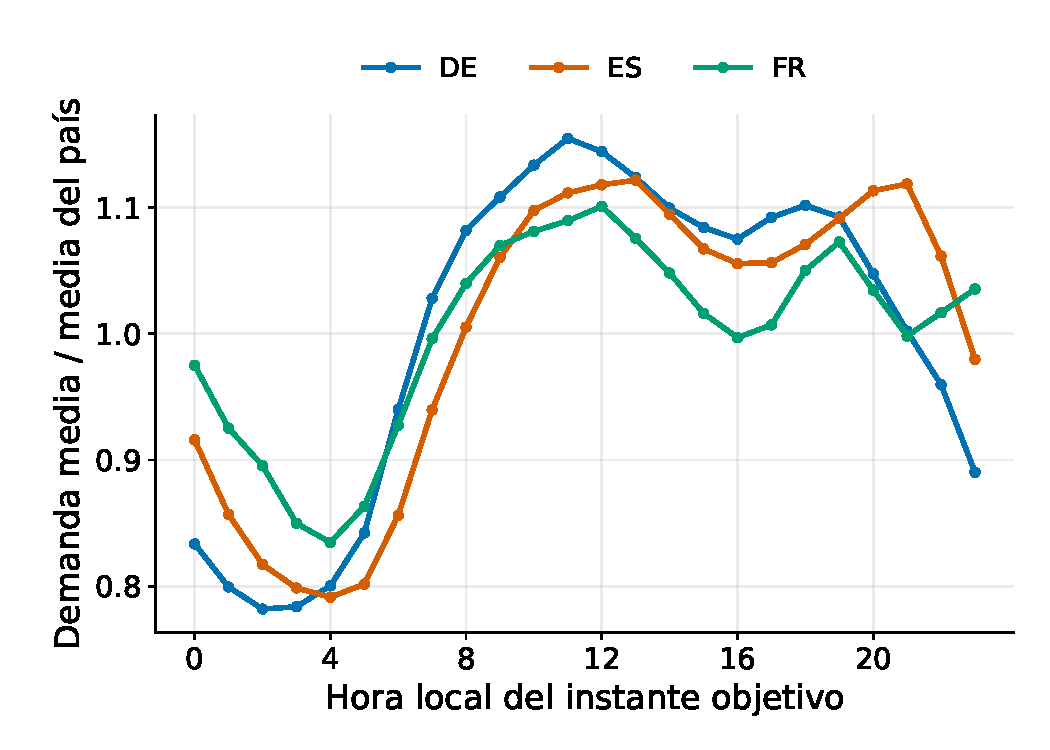
\includegraphics[width=\linewidth,height=0.38\textheight,keepaspectratio]{perfil_hora.pdf}\\[0.3cm]
      \begin{tikzpicture}[font=\footnotesize]
        \node[draw,rounded corners,fill=azulacento!10,minimum width=1.6cm,minimum height=0.8cm] (t) {$t$};
        \node[draw,rounded corners,fill=naranjaoscuro!10,minimum width=1.6cm,minimum height=0.8cm,right=2.1cm of t] (t24) {$t+24$};
        \draw[-{Stealth[length=2.5mm]},thick,azulacento] (t) -- (t24) node[midway,above]{24 h};
        \node[below=0.1cm of t,grisreferencia,font=\tiny] {emisión};
        \node[below=0.1cm of t24,grisreferencia,font=\tiny] {objetivo};
      \end{tikzpicture}
    \end{column}
  \end{columns}
\end{frame}

\begin{frame}{Datos y construcción de la muestra}
  \begin{columns}[T]
    \begin{column}{0.52\textwidth}
      \small
      \begin{itemize}
        \item Fuente: ENTSO-E / Open Power System Data (OPSD).
        \item 43\,824 horas originales (2015--2019), sin duplicados ni ausentes en DE.
        \item Formato largo: $3\times 43\,824=131\,472$ filas país--hora.
        \item Respuesta $Y_{t+24}$ por unión según país e instante objetivo.
        \item Sin imputación: se usan solo \textbf{casos completos}.
        \item \textbf{Desarrollo (2015--2018):} 103\,680 casos completos.
        \item \textbf{Reserva (2019):} 26\,031 casos completos.
      \end{itemize}
    \end{column}
    \begin{column}{0.48\textwidth}
      \centering
      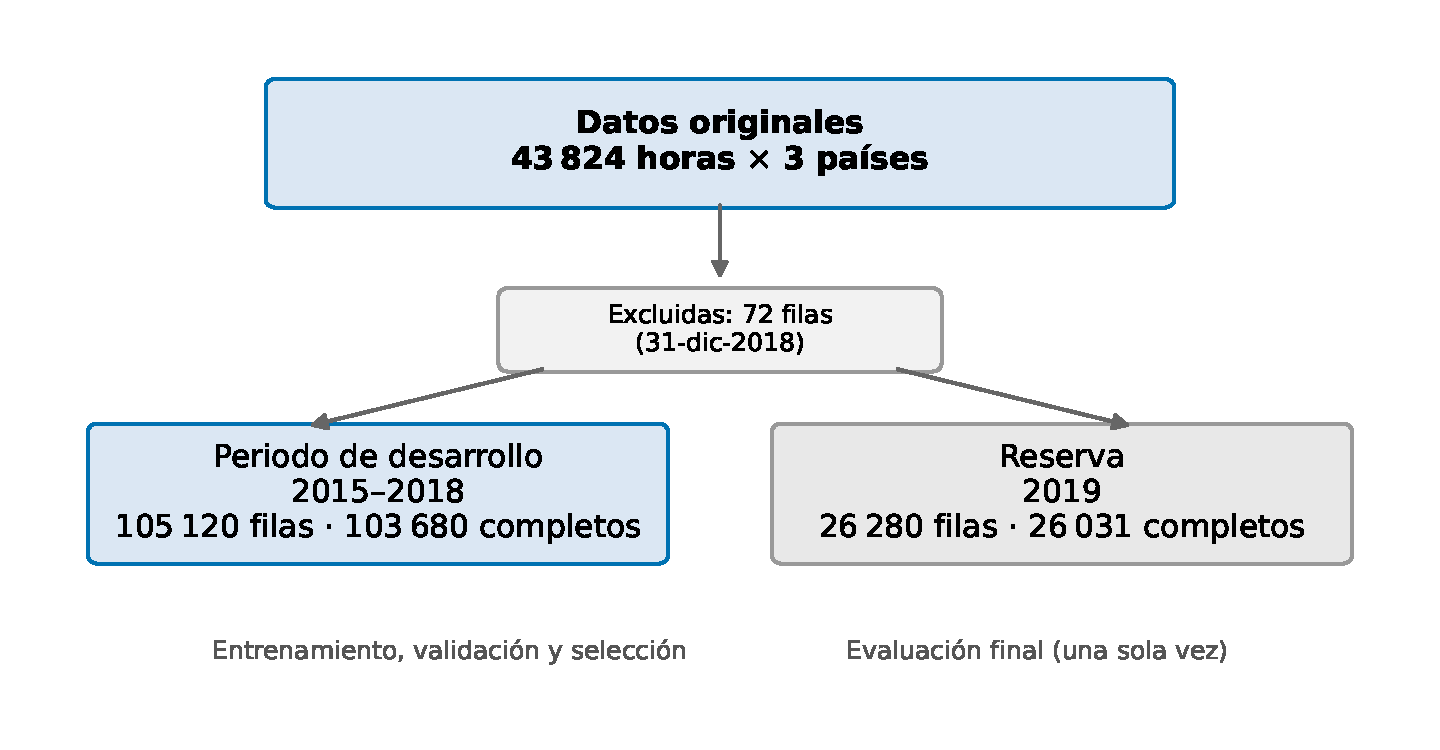
\includegraphics[width=\linewidth,height=0.6\textheight,keepaspectratio]{flujo_muestra.pdf}
    \end{column}
  \end{columns}
\end{frame}

%%%%%%%%%%%%%%%%%%%%%%%%%%%%%%%%%%%%%%%%%%%%%%%%%%%%%%%%%%%%%%%
% SECCIÓN 2. Diseño de validación, información admisible y referencia
%%%%%%%%%%%%%%%%%%%%%%%%%%%%%%%%%%%%%%%%%%%%%%%%%%%%%%%%%%%%%%%
\section{2. Diseño y referencia}

\begin{frame}{Diseño de validación temporal}
  \begin{columns}[T]
    \begin{column}{0.46\textwidth}
      \small
      \begin{itemize}
        \item Tres ventanas de origen creciente W1--W3 dentro del periodo de desarrollo (2015--2018).
        \item Entrenamiento y validación respetan el orden temporal; se reajusta y valida en cada año sucesivo.
        \item Franja de 24 h antes de cada validación excluida del entrenamiento (evita fuga).
        \item Fijados hiperparámetros, se reajusta con 2015--2018 completo.
        \item La \textbf{reserva 2019} se usa una sola vez, al final.
      \end{itemize}
    \end{column}
    \begin{column}{0.54\textwidth}
      \centering
      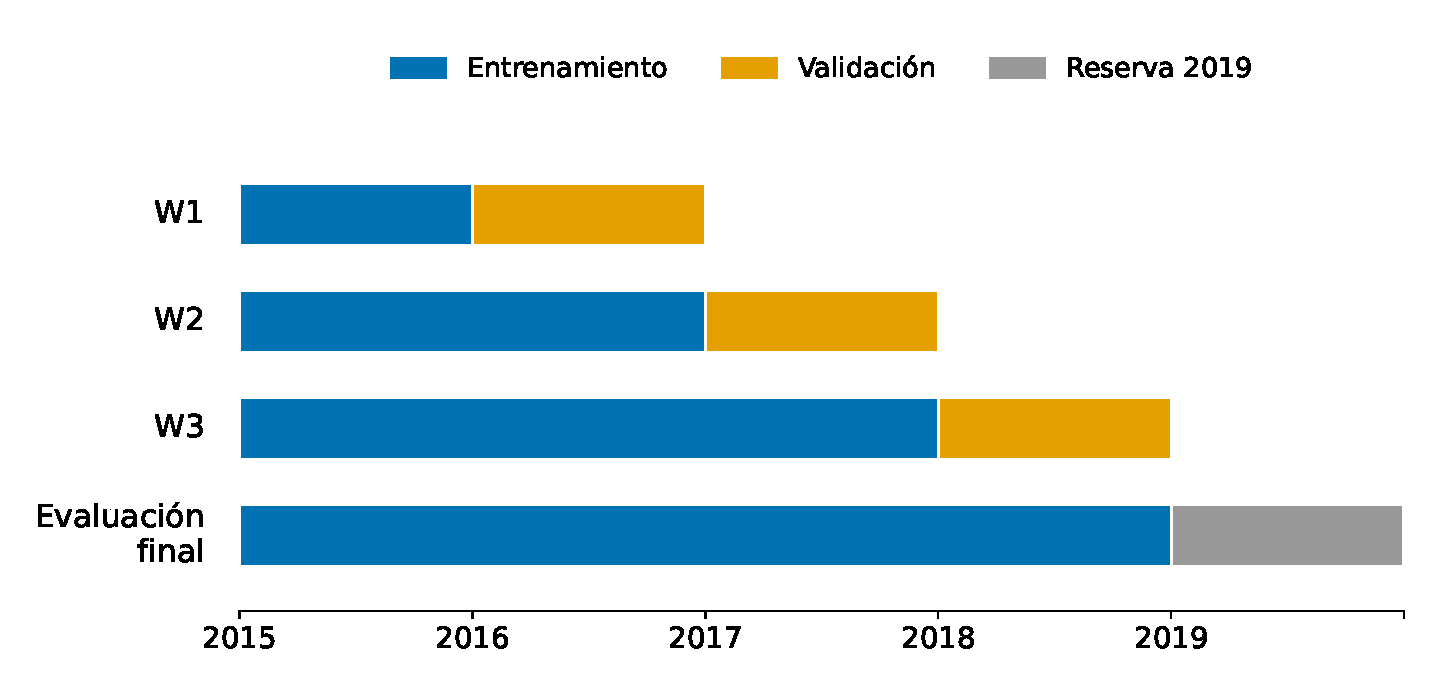
\includegraphics[width=\linewidth,height=0.6\textheight,keepaspectratio]{validacion_temporal.pdf}
    \end{column}
  \end{columns}
\end{frame}

\begin{frame}{Predictores, referencias y métrica}
  \begin{columns}[T]
    \begin{column}{0.55\textwidth}
      \tablafit{generated/tabla_variables}
      \vspace{0.3cm}
      \begin{itemize}
        \item Admisible: se conoce en $t$ (historia de demanda y calendario local determinista de $t+24$).
        \item Referencias: persistencia ($\widehat Y_{t+24}=Y_t$) y \textbf{estacional semanal} ($\widehat Y_{t+24}=Y_{t+24-168}$).
      \end{itemize}
    \end{column}
    \begin{column}{0.45\textwidth}
      \[
        \mathrm{NMAE}_{c,w}=\frac{\mathrm{MAE}_{c,w}}{\overline{Y}_{c,\mathrm{train}(w)}}
      \]
      \[
        \mathrm{NMAE}^{\mathrm{macro}}_{w}=\frac{1}{3}\sum_{c}\mathrm{NMAE}_{c,w}
      \]
      \begin{alertblock}{Referencia semanal (desarrollo)}
        NMAE macro $= 0{,}0537$
      \end{alertblock}
    \end{column}
  \end{columns}
\end{frame}

%%%%%%%%%%%%%%%%%%%%%%%%%%%%%%%%%%%%%%%%%%%%%%%%%%%%%%%%%%%%%%%
% SECCIÓN 3. Métodos, comparación de resultados y diagnóstico
%%%%%%%%%%%%%%%%%%%%%%%%%%%%%%%%%%%%%%%%%%%%%%%%%%%%%%%%%%%%%%%
\section{3. Métodos y resultados}

\begin{frame}{Métodos y resultados en validación}
  \begin{columns}[T]
    \begin{column}{0.42\textwidth}
      \small
      \begin{itemize}
        \item \textbf{Ridge} (M1): lineal, penalización $\ell_2$.
        \item \textbf{Árbol podado} (M2): poda por costo--complejidad.
        \item \textbf{Random Forest} (M3): 200 árboles, indicadores de calendario.
        \item \textbf{Random Forest cíclico} (M3$^\ast$): calendario con seno--coseno.
        \item Comparados con persistencia y referencia semanal.
      \end{itemize}
      \vspace{-0.15cm}
      \begin{alertblock}{Mejor procedimiento (desarrollo)}
        RF cíclico: NMAE $=0{,}0271$\\
        Mejora de 49{,}6\,\% vs. referencia semanal
      \end{alertblock}
    \end{column}
    \begin{column}{0.58\textwidth}
      \centering
      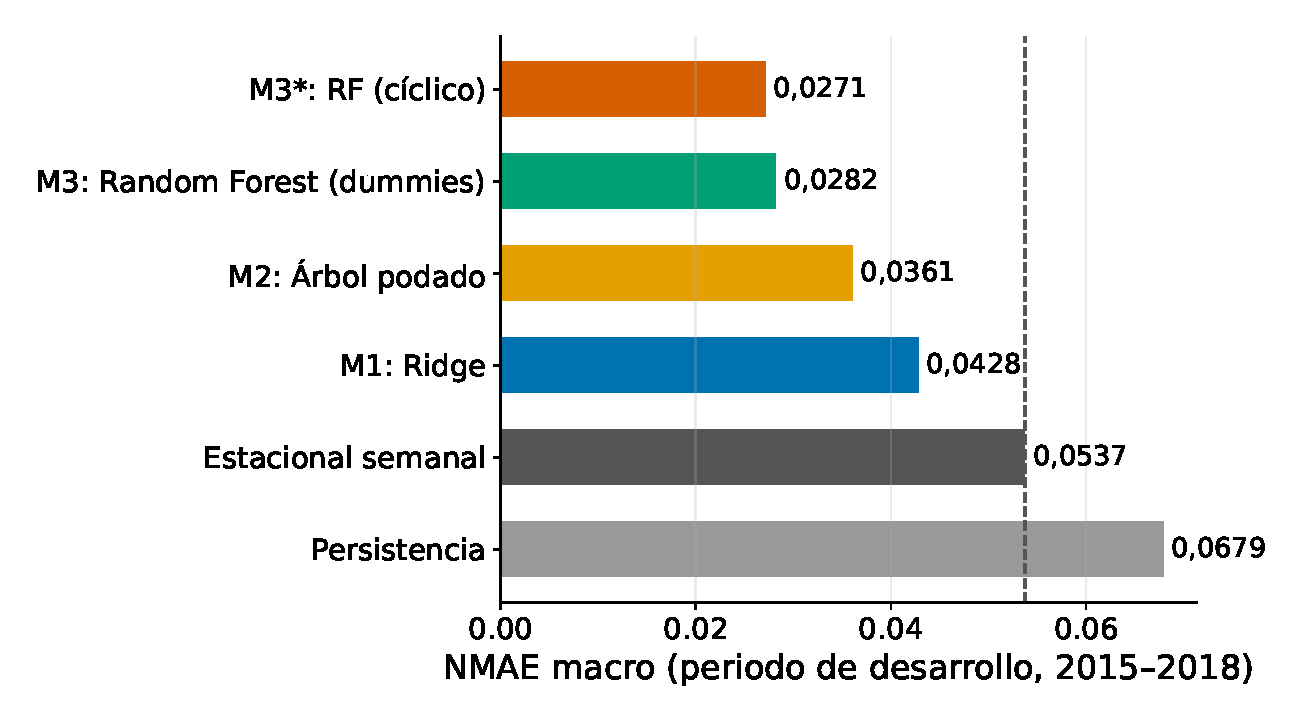
\includegraphics[width=\linewidth,height=0.6\textheight,keepaspectratio]{comparacion_modelos_desarrollo.pdf}
    \end{column}
  \end{columns}
\end{frame}

\begin{frame}{Evaluación final en la reserva 2019}
  \begin{columns}[T]
    \begin{column}{0.55\textwidth}
      \centering
      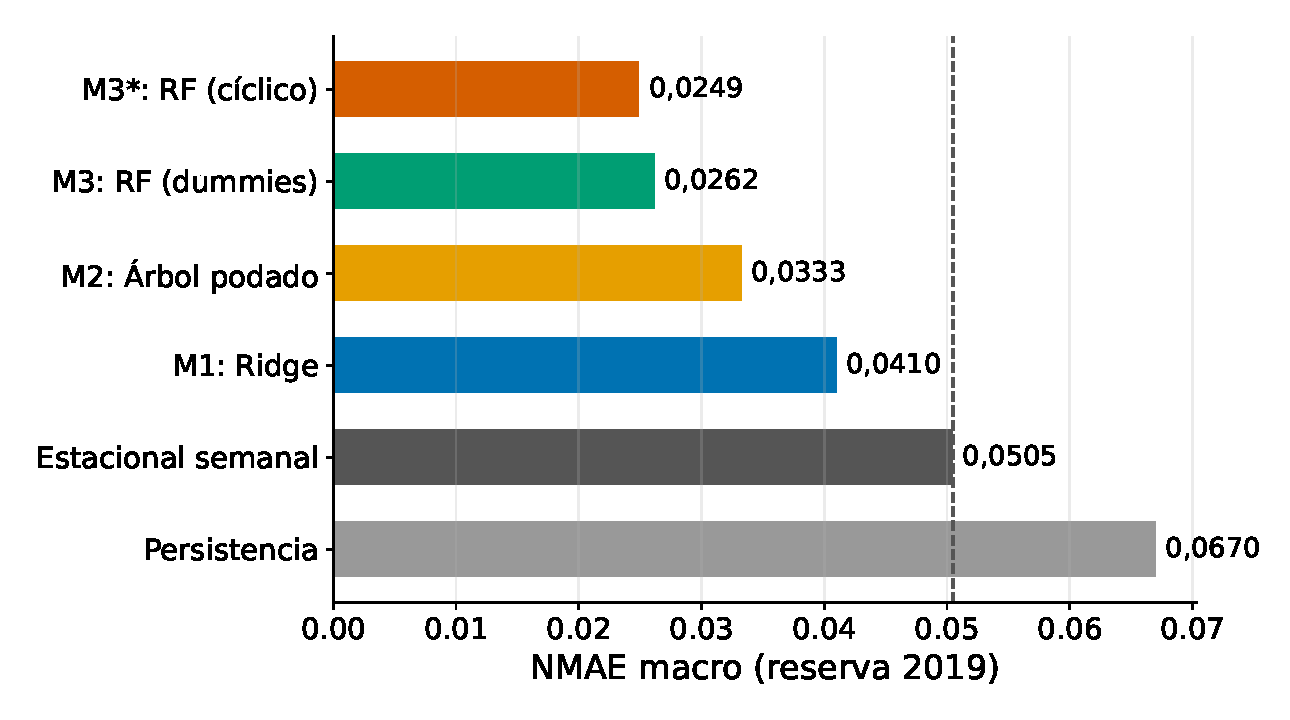
\includegraphics[width=\linewidth,height=0.55\textheight,keepaspectratio]{comparacion_modelos_2019.pdf}
    \end{column}
    \begin{column}{0.45\textwidth}
      \tablafit{generated/resultados_paises}
      \vspace{0.25cm}
      \begin{itemize}
        \item RF cíclico: NMAE $=0{,}0249$ vs. $0{,}0505$ de la referencia.
        \item \textbf{Reducción de 50{,}7\,\%} (IC 95\,\%: 45{,}4\,\%--54{,}9\,\%).
      \end{itemize}
    \end{column}
  \end{columns}
  \vspace{0.15cm}
  {\footnotesize\color{grisreferencia} Resultados de la \textbf{reserva 2019}, no usados para elegir nada; distintos de los resultados de desarrollo (2015--2018) de la diapositiva anterior.}
\end{frame}

\begin{frame}{Diagnóstico de errores}
  \begin{columns}[T]
    \begin{column}{0.55\textwidth}
      \centering
      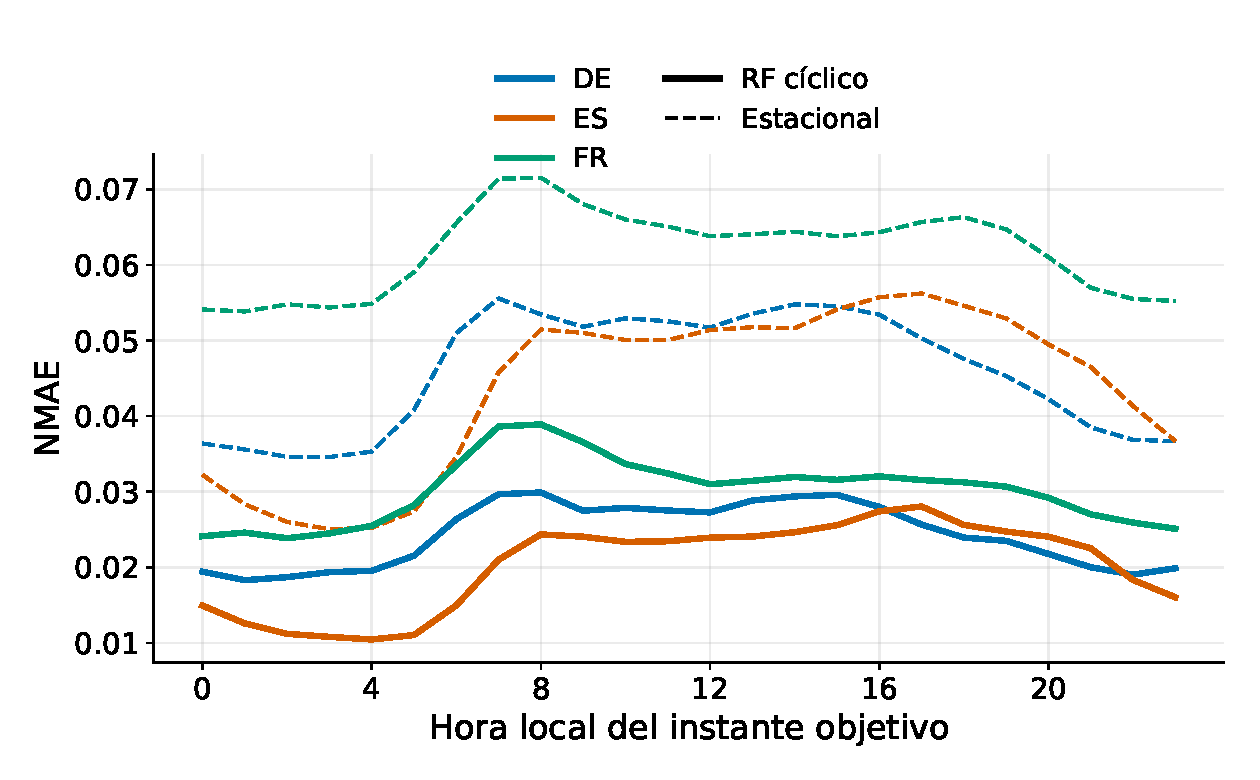
\includegraphics[width=\linewidth,height=0.6\textheight,keepaspectratio]{error_por_hora.pdf}
    \end{column}
    \begin{column}{0.45\textwidth}
      \small
      \begin{itemize}
        \item El RF cíclico supera a la referencia en las 24 horas de los tres países.
        \item Mayor error entre las 8 y las 17 h (horas de alta actividad).
        \item \textbf{Subestima} en alta demanda (sesgo medio):
        \begin{itemize}
          \item DE: $-745$ MW
          \item ES: $-456$ MW
          \item FR: $-920$ MW
        \end{itemize}
        \item Peores días: feriados. MAE diario máximo $=11\,240$ MW (DE, 3 oct. 2019).
      \end{itemize}
    \end{column}
  \end{columns}
\end{frame}

%%%%%%%%%%%%%%%%%%%%%%%%%%%%%%%%%%%%%%%%%%%%%%%%%%%%%%%%%%%%%%%
% SECCIÓN 4. Sensibilidad, recomendación, límites y reproducibilidad
%%%%%%%%%%%%%%%%%%%%%%%%%%%%%%%%%%%%%%%%%%%%%%%%%%%%%%%%%%%%%%%
\section{4. Sensibilidad y cierre}

\begin{frame}{Análisis de sensibilidad}
  \begin{columns}[T]
    \begin{column}{0.5\textwidth}
      \centering
      {\small\textbf{S1: representación del calendario}}\\[0.15cm]
      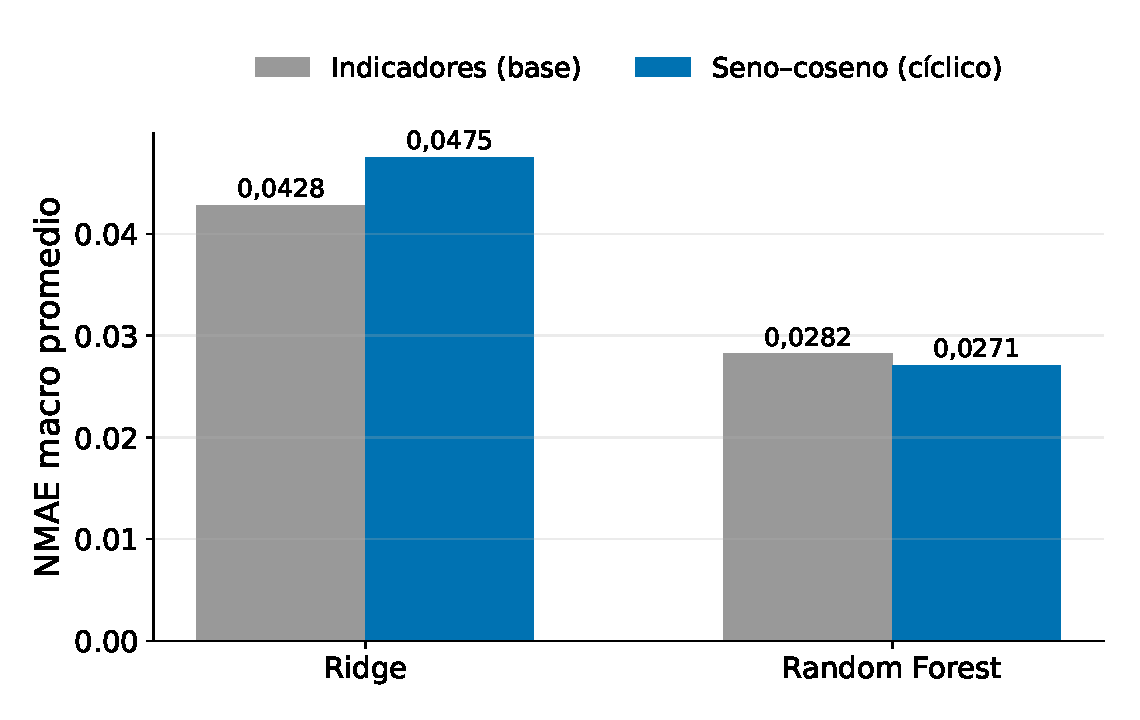
\includegraphics[width=\linewidth,height=0.4\textheight,keepaspectratio]{sensibilidad_calendario.pdf}\\[0.1cm]
      {\footnotesize RF: $0{,}0282\to 0{,}0271$ (mejora 3{,}9\,\%)}
    \end{column}
    \begin{column}{0.5\textwidth}
      \centering
      {\small\textbf{S2: historia de entrenamiento}}\\[0.15cm]
      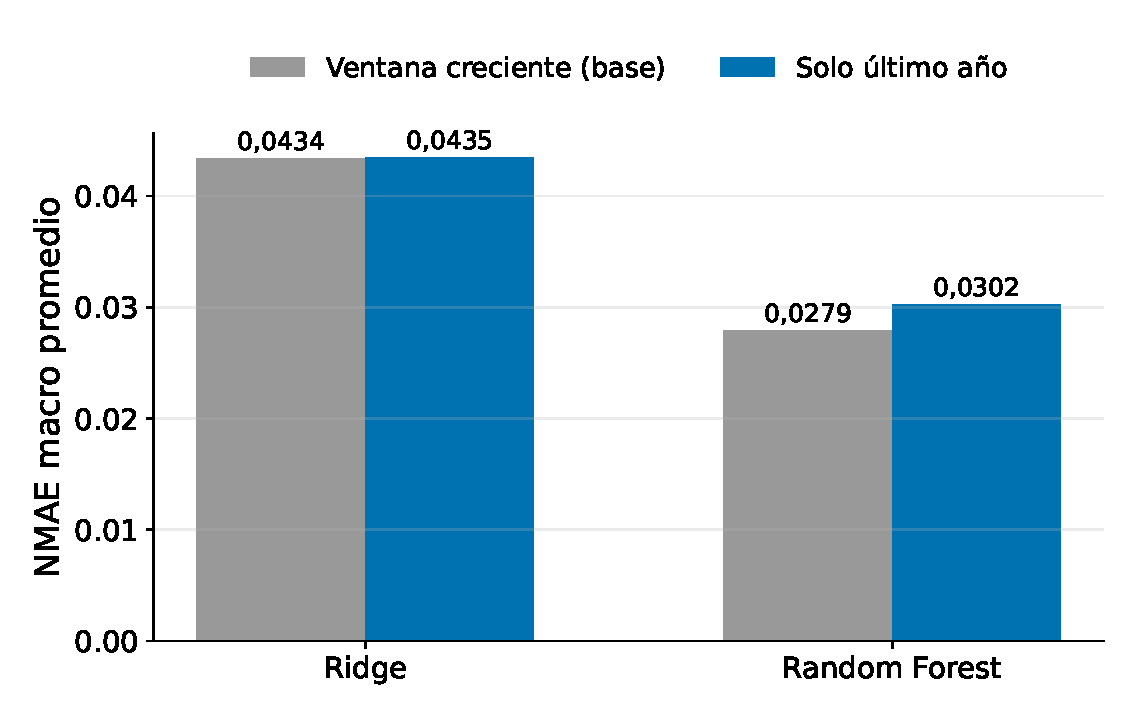
\includegraphics[width=\linewidth,height=0.4\textheight,keepaspectratio]{sensibilidad_historia.pdf}\\[0.1cm]
      {\footnotesize RF: $0{,}0279\to 0{,}0302$ (empeora 8{,}3\,\%)}
    \end{column}
  \end{columns}
  \vspace{0.2cm}
  {\footnotesize\color{grisreferencia} Ambos análisis se evalúan solo en el periodo de desarrollo (2015--2018). S2 usa el promedio de W2 y W3 (W1 solo tiene un año de historia disponible).}
\end{frame}

\begin{frame}{Recomendación y limitaciones}
  \begin{columns}[T]
    \begin{column}{0.33\textwidth}
      \begin{block}{Recomendación}
        \begin{itemize}
          \item Usar RF cíclico.
          \item Reajustar periódicamente con toda la historia disponible.
          \item Monitorear frente a la referencia semanal.
        \end{itemize}
      \end{block}
    \end{column}
    \begin{column}{0.33\textwidth}
      \begin{block}{Condiciones}
        \begin{itemize}
          \item Últimas 168 h de demanda sin faltantes.
          \item Calendario local del instante objetivo.
        \end{itemize}
      \end{block}
    \end{column}
    \begin{column}{0.34\textwidth}
      \begin{block}{Limitaciones}
        \begin{itemize}
          \item Sin temperatura ni feriados.
          \item Error alto en feriados y día posterior.
          \item Subestima en demanda extrema.
          \item Evaluación final: solo 2019.
          \item No garantiza generalizar a otros períodos/países.
        \end{itemize}
      \end{block}
    \end{column}
  \end{columns}
\end{frame}

\begin{frame}{Reproducibilidad}
  \begin{columns}[T]
    \begin{column}{0.55\textwidth}
      \small
      \begin{itemize}
        \item Repositorio público del proyecto (GitHub).
        \item Ejecución completa: \texttt{python analisis.py} (auditoría, base analítica, validación, sensibilidades, evaluación 2019, bootstrap, diagnóstico, tablas y figuras).
        \item Dependencias fijas (\texttt{requirements.txt}) y semilla fija (\texttt{random\_state=42}).
        \item Tiempo de ejecución integrada: 12{,}2 minutos.
        \item Comprobación de concordancia frente a resultados previos (\texttt{results/concordancia.csv}).
        \item Ejecución en copia limpia (mismo equipo): 13{,}8 minutos, misma concordancia.
      \end{itemize}
    \end{column}
    \begin{column}{0.45\textwidth}
      \centering
      \begin{tikzpicture}[font=\footnotesize,
          caja/.style={draw,rounded corners,fill=azulacento!8,text width=2.7cm,align=center,inner sep=2pt}]
        \node[caja] (datos) {Datos originales\\\texttt{data/raw/}};
        \node[caja,below=0.08cm of datos] (base) {Base analítica\\y validación};
        \node[caja,below=0.08cm of base] (res) {\texttt{results/}};
        \node[caja,below=0.08cm of res] (pres) {Tablas y figuras\\de esta presentación};
        \draw[-{Stealth[length=2mm]},azulacento] (datos) -- (base);
        \draw[-{Stealth[length=2mm]},azulacento] (base) -- (res);
        \draw[-{Stealth[length=2mm]},azulacento] (res) -- (pres);
      \end{tikzpicture}
    \end{column}
  \end{columns}
\end{frame}

%%%%%%%%%%%%%%%%%%%%%%%%%%%%%%%%%%%%%%%%%%%%%%%%%%%%%%%%%%%%%%%
% DIAPOSITIVA 12 --- CIERRE
%%%%%%%%%%%%%%%%%%%%%%%%%%%%%%%%%%%%%%%%%%%%%%%%%%%%%%%%%%%%%%%
\begin{frame}[plain]
  \begin{center}
    \vspace{2.5cm}
    {\usebeamerfont{title}\usebeamercolor[fg]{title}\textbf{Gracias}}\\[0.6cm]
    {\usebeamerfont{subtitle}\color{grafito} Preguntas}
  \end{center}
\end{frame}

%%%%%%%%%%%%%%%%%%%%%%%%%%%%%%%%%%%%%%%%%%%%%%%%%%%%%%%%%%%%%%%
% DIAPOSITIVAS DE RESPALDO (fuera de la exposición principal)
%%%%%%%%%%%%%%%%%%%%%%%%%%%%%%%%%%%%%%%%%%%%%%%%%%%%%%%%%%%%%%%
\appendix
\section{Respaldo}

\begin{frame}{Respaldo: descripción de la demanda}
  \begin{columns}[T]
    \begin{column}{0.55\textwidth}
      \centering
      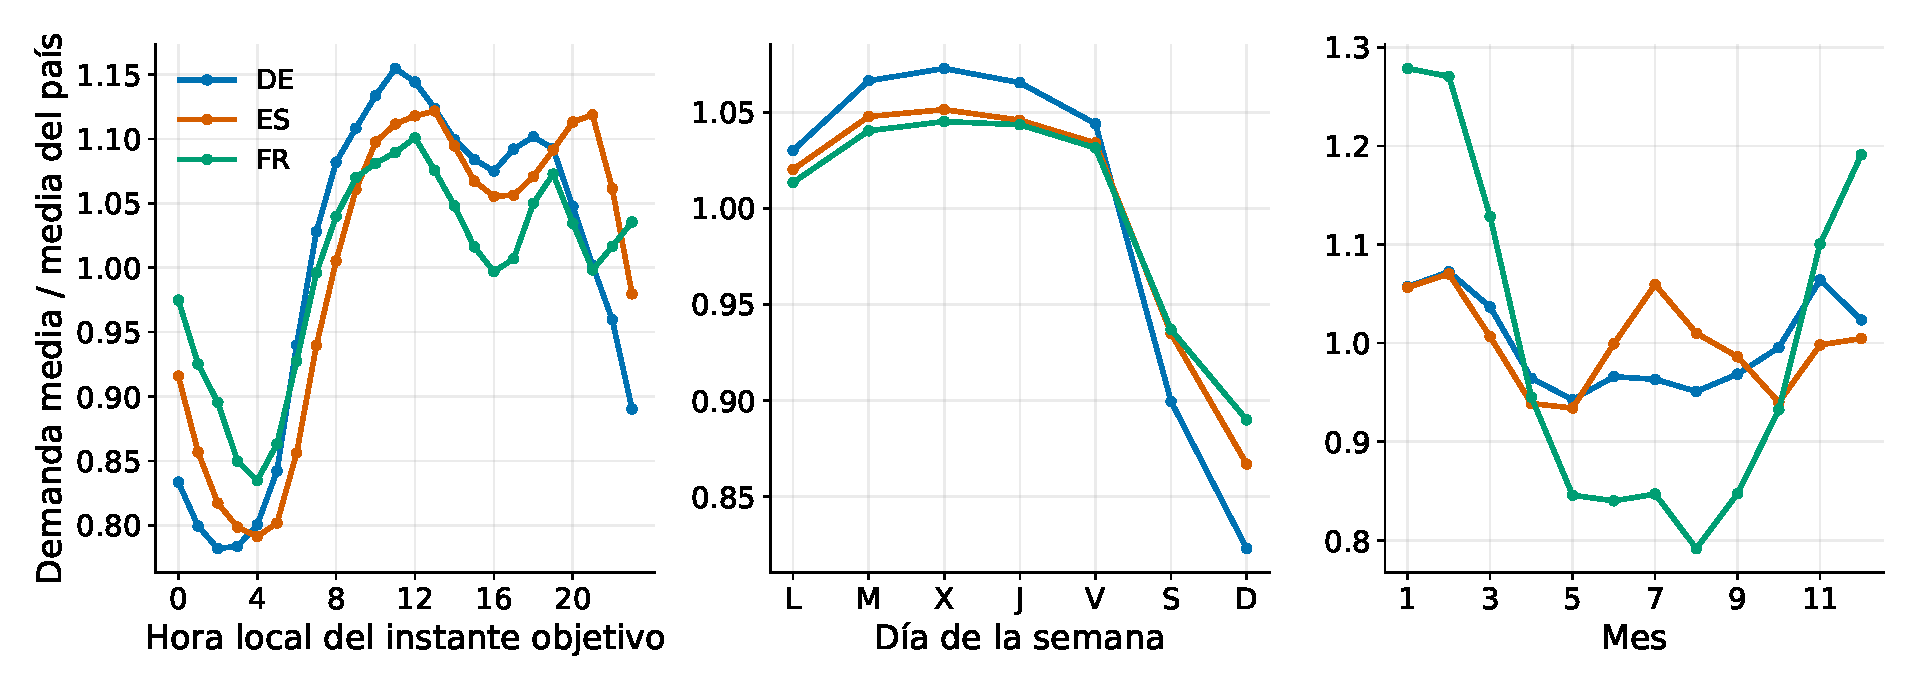
\includegraphics[width=\linewidth,height=0.6\textheight,keepaspectratio]{perfil_demanda.pdf}
    \end{column}
    \begin{column}{0.45\textwidth}
      \tablafit{generated/respaldo/tabla_respuesta}
    \end{column}
  \end{columns}
\end{frame}

\begin{frame}{Respaldo: construcción de muestra y validación}
  \begin{columns}[T]
    \begin{column}{0.4\textwidth}
      \tablafit[3.0cm]{generated/tabla_ventanas}
      \vspace{0.15cm}
      \tablafit[3.0cm]{generated/respaldo/tabla_ausentes_bloques}
    \end{column}
    \begin{column}{0.6\textwidth}
      \tablafit[4.2cm]{generated/respaldo/tabla_ausentes_efecto}
    \end{column}
  \end{columns}
  \vspace{0.05cm}
  \recursopendiente{Tabla 1 del informe (construcción de la muestra por periodo y
  país, \texttt{tab:muestra}) aún no se adaptó a esta biblioteca; ubicación
  esperada si se genera: \texttt{generated/respaldo/tabla\_muestra.tex}.}
\end{frame}

\begin{frame}{Respaldo: hiperparámetros y complejidad}
  \begin{columns}[T]
    \begin{column}{0.5\textwidth}
      \tablafit{generated/respaldo/tabla_rf_busqueda}
    \end{column}
    \begin{column}{0.5\textwidth}
      \tablafit[3.0cm]{generated/respaldo/tabla_complejidad}
      \vspace{0.15cm}
      \tablafit[3.0cm]{generated/respaldo/tabla_tiempos}
    \end{column}
  \end{columns}
  \vspace{0.3cm}
  \recursopendiente{Tabla 4 del informe (procedimientos e hiperparámetros
  evaluados, \texttt{tab:busqueda}) está escrita directamente en
  \texttt{reports/informe/content/metodos.tex} y no se exportó como tabla
  generada; ubicación esperada si se adapta:
  \texttt{generated/respaldo/tabla\_busqueda.tex}.}
\end{frame}

\begin{frame}{Respaldo: resultados detallados por país (1/2)}
  \framesubtitle{Resumen por país y detalle en la reserva 2019}
  \tablafit[3.2cm]{generated/resultados_paises}
  \vspace{0.2cm}
  \tablafit[3.2cm]{generated/respaldo/tabla_test_detalle}
\end{frame}

\begin{frame}{Respaldo: resultados detallados por país (2/2)}
  \framesubtitle{Detalle por ventana de validación en el periodo de desarrollo}
  \tablafit[4.0cm]{generated/respaldo/tabla_detalle}
\end{frame}

\begin{frame}{Respaldo: bootstrap e incertidumbre}
  \begin{columns}[T]
    \begin{column}{0.5\textwidth}
      \centering
      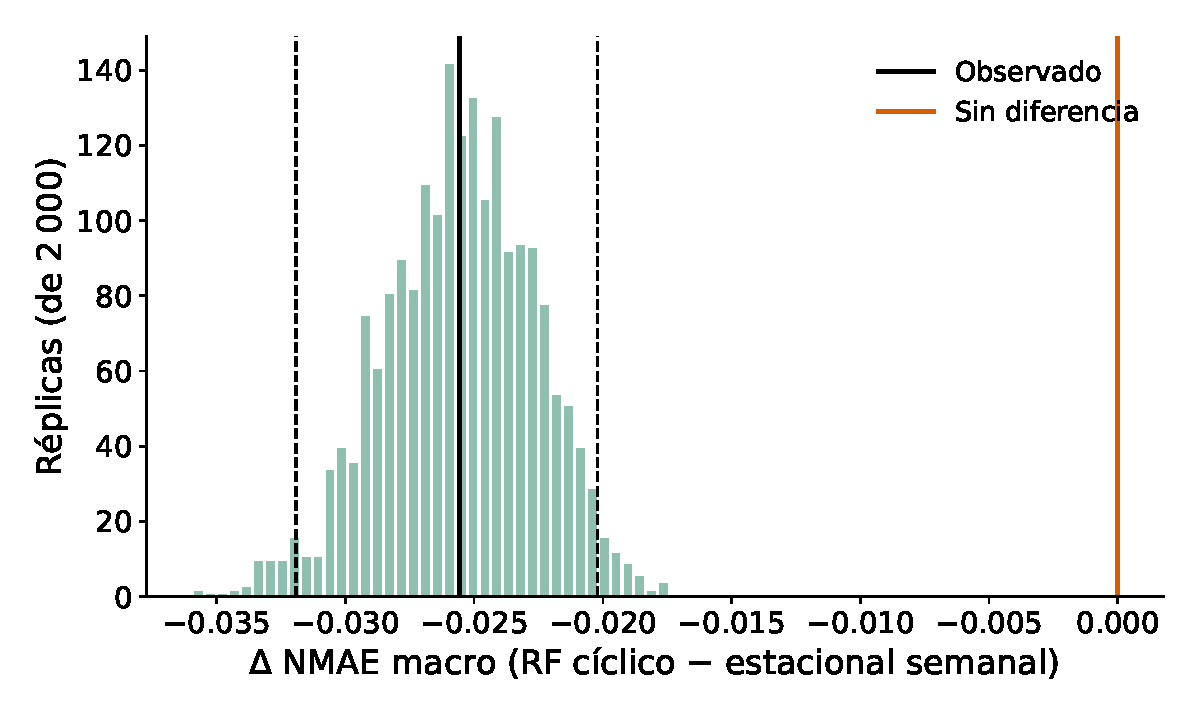
\includegraphics[width=\linewidth,height=0.6\textheight,keepaspectratio]{bootstrap_respaldo.pdf}
    \end{column}
    \begin{column}{0.5\textwidth}
      \tablafit{generated/intervalos_confianza}
    \end{column}
  \end{columns}
\end{frame}

\begin{frame}{Respaldo: importancia de variables y errores extremos}
  \begin{columns}[T]
    \begin{column}{0.5\textwidth}
      \tablafit{generated/respaldo/tabla_importancia}
    \end{column}
    \begin{column}{0.5\textwidth}
      \tablafit{generated/casos_extremos}
    \end{column}
  \end{columns}
\end{frame}

\end{document}
